\section{The Logistic Map}

\begin{frame}{From Continuous to Discrete Time}
  \begin{itemize}
    \item In differential equations, time is a continuous variable $t$.
    \item In a \textbf{discrete-time model}, time advances in steps: $0, 1, 2, 3, \ldots$
    \item Such models work well for organisms with \textbf{well-defined breeding seasons} (fish, insects), or for phenomena with natural cycles (heartbeats, annual measurements).
    \item The governing equation is called a \textbf{difference equation}:
    \[
      X_{N+1} = f(X_N)
    \]
    \item Simplest example: $X_{N+1} = r\,X_N$ (discrete analogue of Malthusian growth).
  \end{itemize}
\end{frame}

\begin{frame}{The Logistic Map}
  \begin{itemize}
    \item Consider a population of insects that live one year, lay eggs, and die.
    \item Resources support a maximum of $K$ individuals.
    \item Current population $X_N$ uses a fraction $\frac{X_N}{K}$ of resources.
    \item The unused fraction $1 - \frac{X_N}{K}$ is available for the next generation.
    \item This gives the \textbf{logistic map}:
    \[
      X_{N+1} = r\,X_N\left(1 - \frac{X_N}{K}\right)
    \]
    \item Setting $K = 1$ (normalised population):
    \[
      X_{N+1} = r\,X_N(1 - X_N)
    \]
    \item The parameter $r \in [0,4]$ keeps $X_N$ bounded in $[0,1]$.
  \end{itemize}
\end{frame}

\begin{frame}{The Logistic Parabola}
  The shape of the map $f(x) = r\,x(1-x)$ depends on $r$:
  \begin{center}
    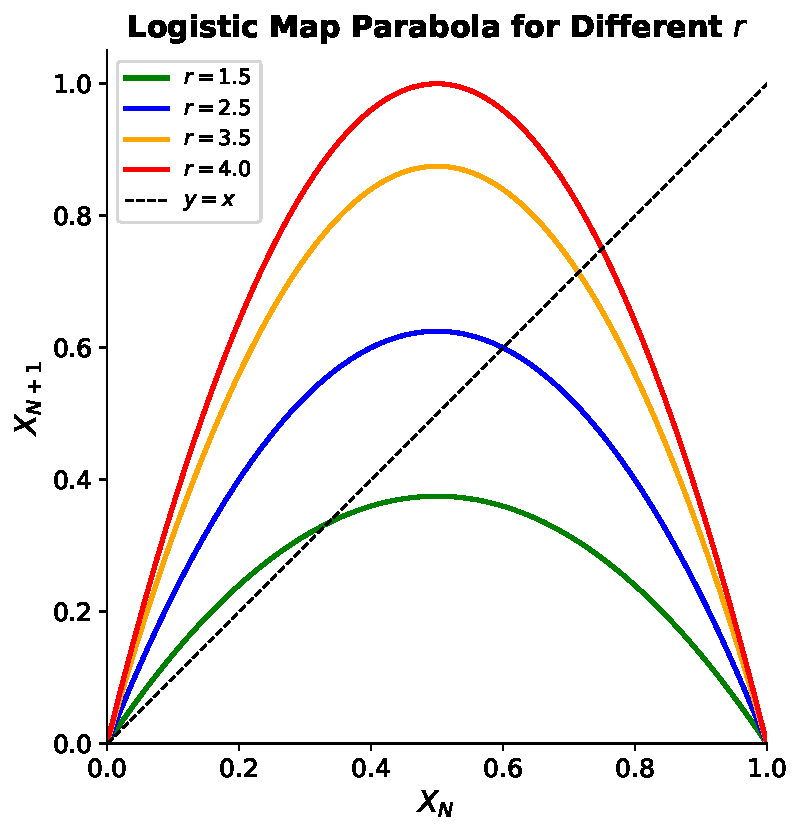
\includegraphics[width=0.55\textwidth]{images/logistic_parabola.pdf}
  \end{center}
  \begin{itemize}
    \item Fixed points lie where the parabola intersects the diagonal $y = x$.
    \item As $r$ grows, the parabola stretches and the dynamics become richer.
  \end{itemize}
\end{frame}

\begin{frame}{Historical Context}
  \begin{itemize}
    \item The logistic map was popularised by the biologist \textbf{Robert May} in 1976.
    \item May showed that this deceptively simple equation can produce extraordinarily complex behaviour.
    \item His paper \textit{``Simple mathematical models with very complicated dynamics''} (Nature, 1976) became one of the most cited papers in mathematical biology.
    \item The logistic map became a key example in the emerging science of \textbf{chaos theory}.
  \end{itemize}
\end{frame}

\begin{frame}{Behaviour for Different Values of $r$}
\small
  \begin{itemize}
    \item $0 < r \leq 1$: Population dies out ($X_N \to 0$).
    \item $1 < r \leq 3$: Population converges to a \textbf{fixed point} $X^* = 1 - \frac{1}{r}$.
    \pause
    \item $3 < r \lesssim 3.449$: Population oscillates between \textbf{two values} (period-2 cycle).
    \item $3.449 \lesssim r \lesssim 3.544$: Population oscillates between \textbf{four values} (period-4 cycle).
    \pause
    \item As $r$ increases further, the period keeps \textbf{doubling}: 8, 16, 32, \ldots
    \item Beyond $r \approx 3.57$: the system enters \textbf{chaos} --- the sequence never repeats.
    \item Within the chaotic regime, there are narrow \textbf{windows of periodicity} (e.g.\ period-3 near $r \approx 3.83$).
  \end{itemize}
\end{frame}

\begin{frame}{Time Series for Different $r$}
  \begin{center}
    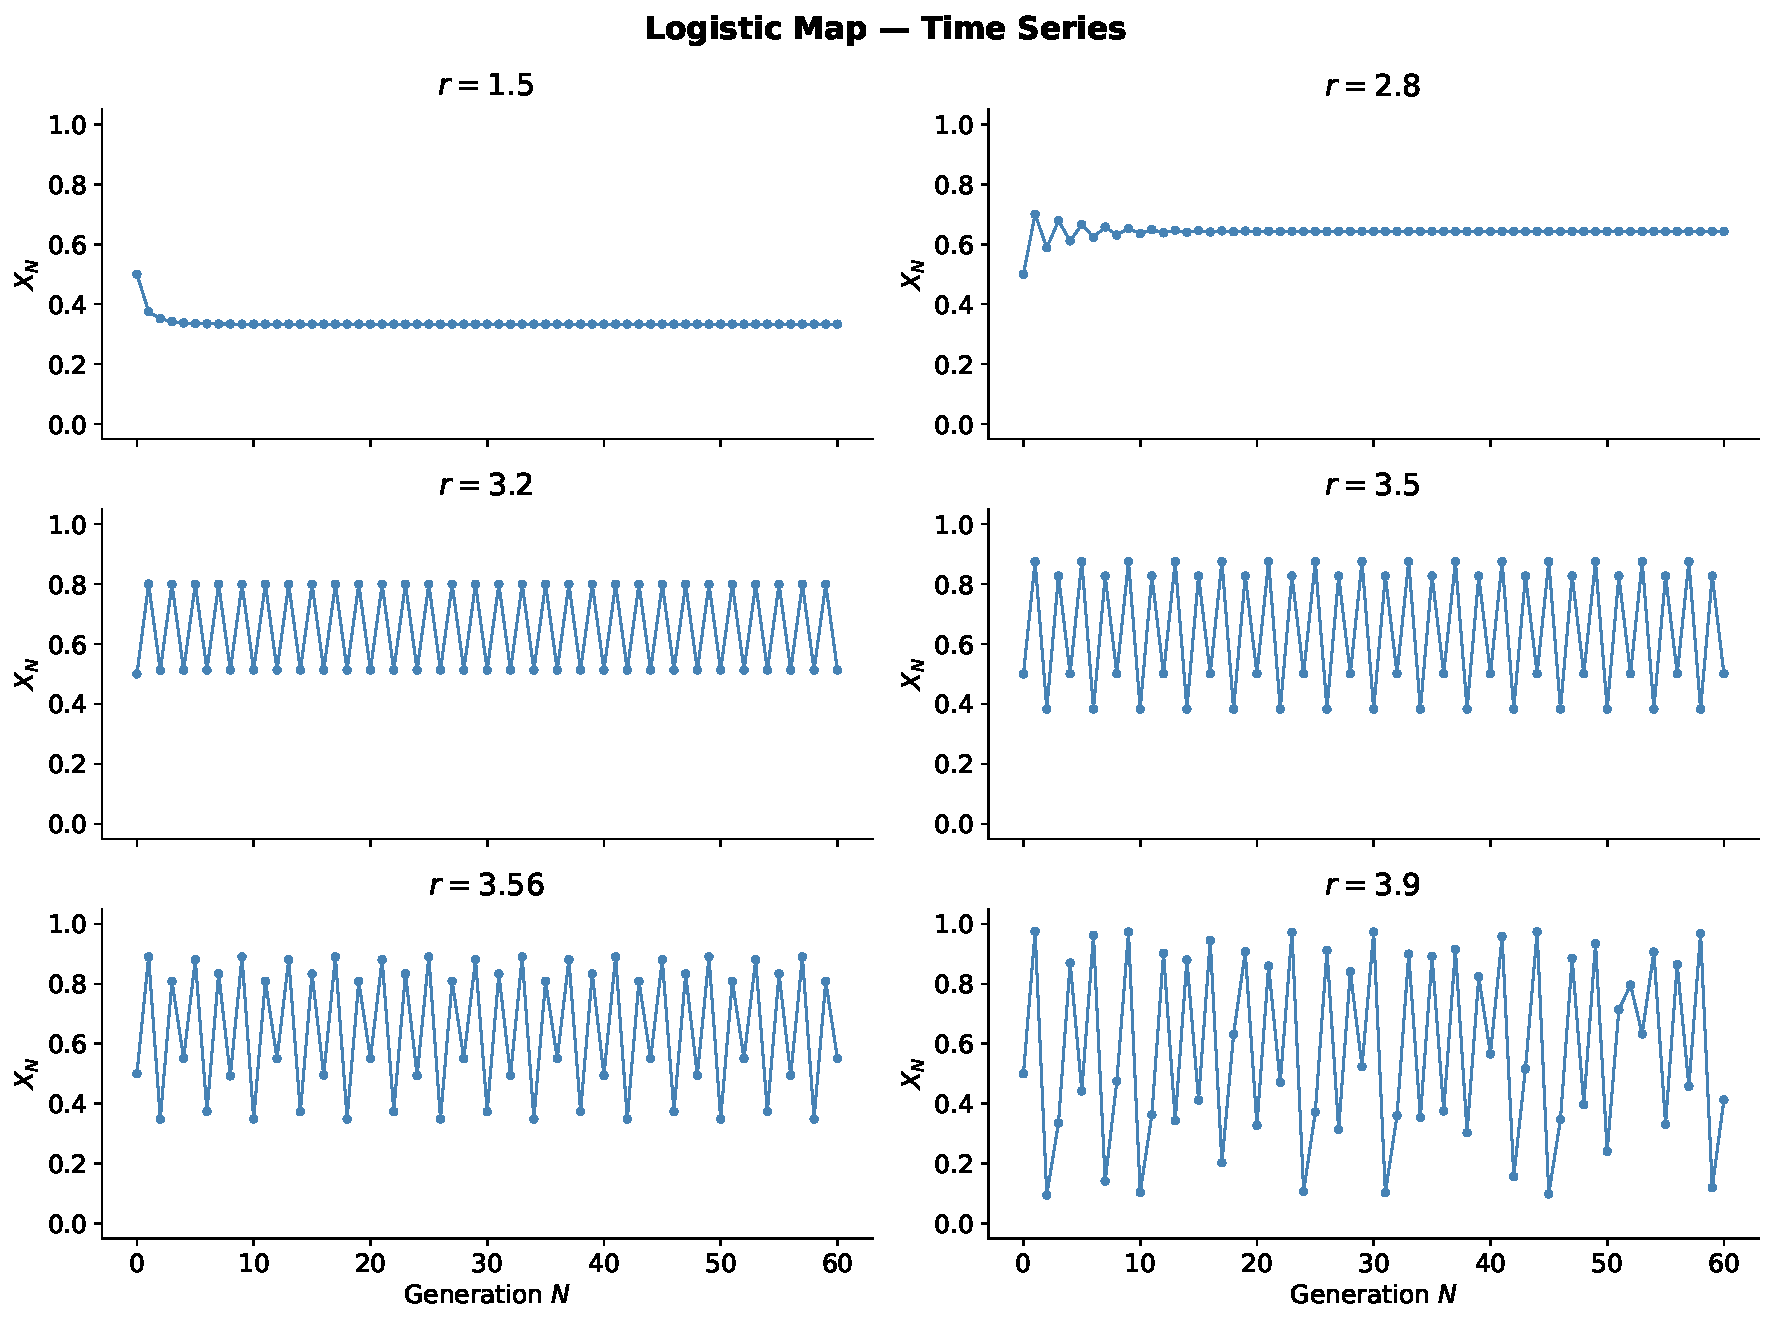
\includegraphics[width=0.92\textwidth]{images/logistic_timeseries.pdf}
  \end{center}
\end{frame}

% ---- TikZ Cobweb: Stable fixed point (r = 2.5) ----
\begin{frame}{Cobweb Diagram --- Stable Fixed Point}
  \begin{columns}
    \column{0.55\textwidth}
    \begin{center}
    \begin{tikzpicture}[scale=5.5, declare function={f(\x)=2.5*\x*(1-\x);}]
        \draw[thin, color=gray!40, step=0.1] (0,0) grid (1,1);
        \draw[very thick,-](0,1)|-(1,0);
        \draw[very thick, green!70!black] (0,0)--(1,1);
        \draw[very thick, blue, domain=0:1, smooth] plot (\x,{f(\x)});
        \pgfmathsetmacro{\startv}{0.2}
        \draw[very thick,red] (\startv,0) -- (\startv,\startv);
        \foreach \t[evaluate=\t as \newv using f(\startv)] in {1,...,20}{%
            \draw[very thick, red] (\startv,\startv)|-(\newv,\newv);%
            \xdef\startv{\newv}%
        }
        \node at (0.5, -0.06) {\small$X_{N}$};
        \node at (-0.06, 0.5) [rotate=90] {\small$X_{N+1}$};
    \end{tikzpicture}
    \end{center}
    \column{0.45\textwidth}
    \begin{itemize}
      \item $r = 2.5$, $X_0 = 0.2$
      \item The cobweb \textbf{spirals inward} to the fixed point $X^* = 0.6$.
      \item The fixed point is \textbf{stable}.
    \end{itemize}
  \end{columns}
\end{frame}

% ---- TikZ Cobweb: Period-2 (r = 3.2) ----
\begin{frame}{Cobweb Diagram --- Period-2 Cycle}
  \begin{columns}
    \column{0.55\textwidth}
    \begin{center}
    \begin{tikzpicture}[scale=5.5, declare function={f(\x)=3.2*\x*(1-\x);}]
        \draw[thin, color=gray!40, step=0.1] (0,0) grid (1,1);
        \draw[very thick,-](0,1)|-(1,0);
        \draw[very thick, green!70!black] (0,0)--(1,1);
        \draw[very thick, blue, domain=0:1, smooth] plot (\x,{f(\x)});
        \pgfmathsetmacro{\startv}{0.2}
        \draw[very thick,red] (\startv,0) -- (\startv,\startv);
        \foreach \t[evaluate=\t as \newv using f(\startv)] in {1,...,30}{%
            \draw[very thick, red] (\startv,\startv)|-(\newv,\newv);%
            \xdef\startv{\newv}%
        }
        \node at (0.5, -0.06) {\small$X_{N}$};
        \node at (-0.06, 0.5) [rotate=90] {\small$X_{N+1}$};
    \end{tikzpicture}
    \end{center}
    \column{0.45\textwidth}
    \begin{itemize}
      \item $r = 3.2$, $X_0 = 0.2$
      \item The cobweb settles into a \textbf{rectangle}, alternating between two values.
      \item This is a \textbf{period-2 cycle}.
    \end{itemize}
  \end{columns}
\end{frame}

% ---- TikZ Cobweb: Chaos (r = 3.9) ----
\begin{frame}{Cobweb Diagram --- Chaos}
  \begin{columns}
    \column{0.55\textwidth}
    \begin{center}
    \begin{tikzpicture}[scale=5.5, declare function={f(\x)=3.9*\x*(1-\x);}]
        \draw[thin, color=gray!40, step=0.1] (0,0) grid (1,1);
        \draw[very thick,-](0,1)|-(1,0);
        \draw[very thick, green!70!black] (0,0)--(1,1);
        \draw[very thick, blue, domain=0:1, smooth] plot (\x,{f(\x)});
        \pgfmathsetmacro{\startv}{0.2}
        \draw[very thick,red] (\startv,0) -- (\startv,\startv);
        \foreach \t[evaluate=\t as \newv using f(\startv)] in {1,...,30}{%
            \draw[very thick, red] (\startv,\startv)|-(\newv,\newv);%
            \xdef\startv{\newv}%
        }
        \node at (0.5, -0.06) {\small$X_{N}$};
        \node at (-0.06, 0.5) [rotate=90] {\small$X_{N+1}$};
    \end{tikzpicture}
    \end{center}
    \column{0.45\textwidth}
    \begin{itemize}
      \item $r = 3.9$, $X_0 = 0.2$
      \item The cobweb fills the entire space \textbf{irregularly}.
      \item No pattern repeats --- this is \textbf{chaos}.
    \end{itemize}
  \end{columns}
\end{frame}

% ---- Python cobweb comparison ----
\begin{frame}{Cobweb Diagrams --- All Regimes at a Glance}
  \begin{center}
    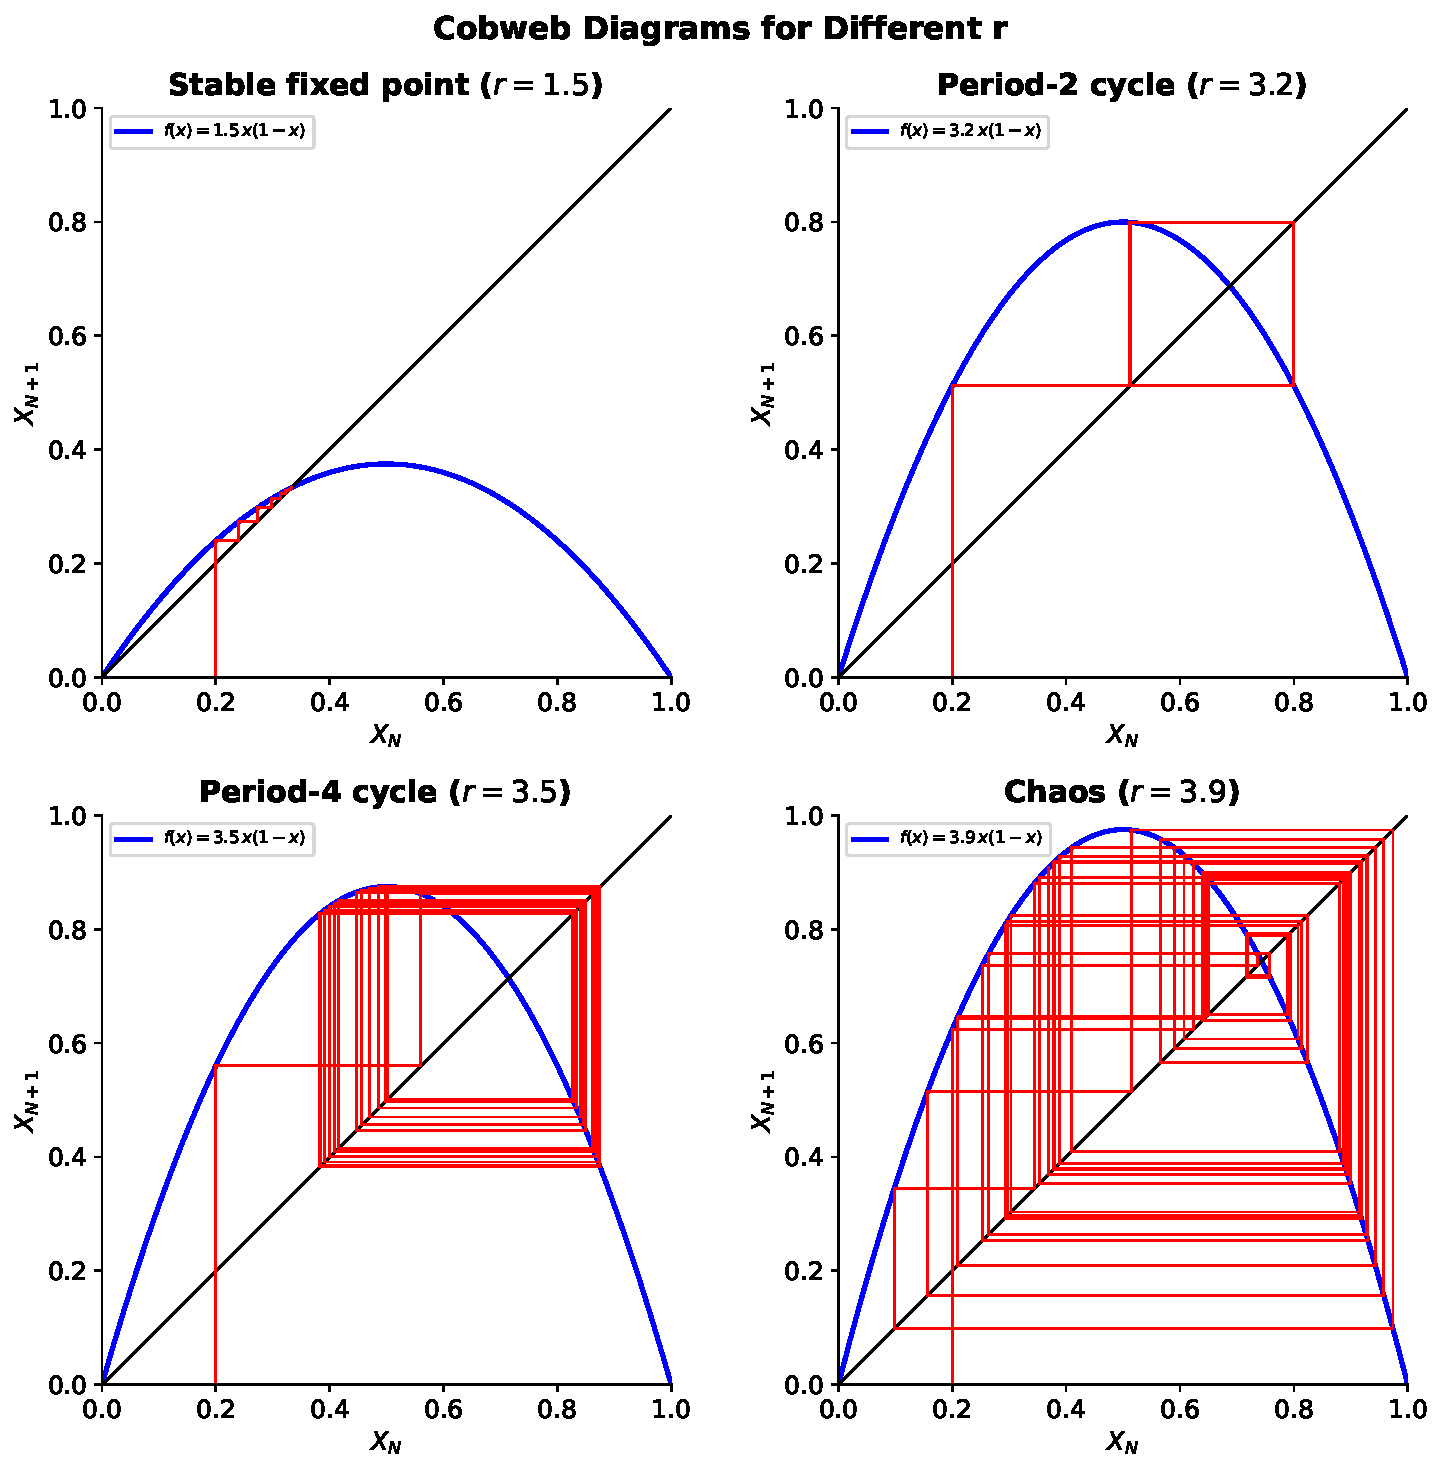
\includegraphics[width=0.88\textwidth]{images/cobweb_combined.pdf}
  \end{center}
\end{frame}

\begin{frame}{The Bifurcation Diagram}
  \begin{itemize}
    \item The \textbf{bifurcation diagram} summarises all possible long-term behaviours as $r$ varies.
    \item For each value of $r$, iterate many times to remove transients, then plot the visited values of $X$.
  \end{itemize}
  \begin{center}
    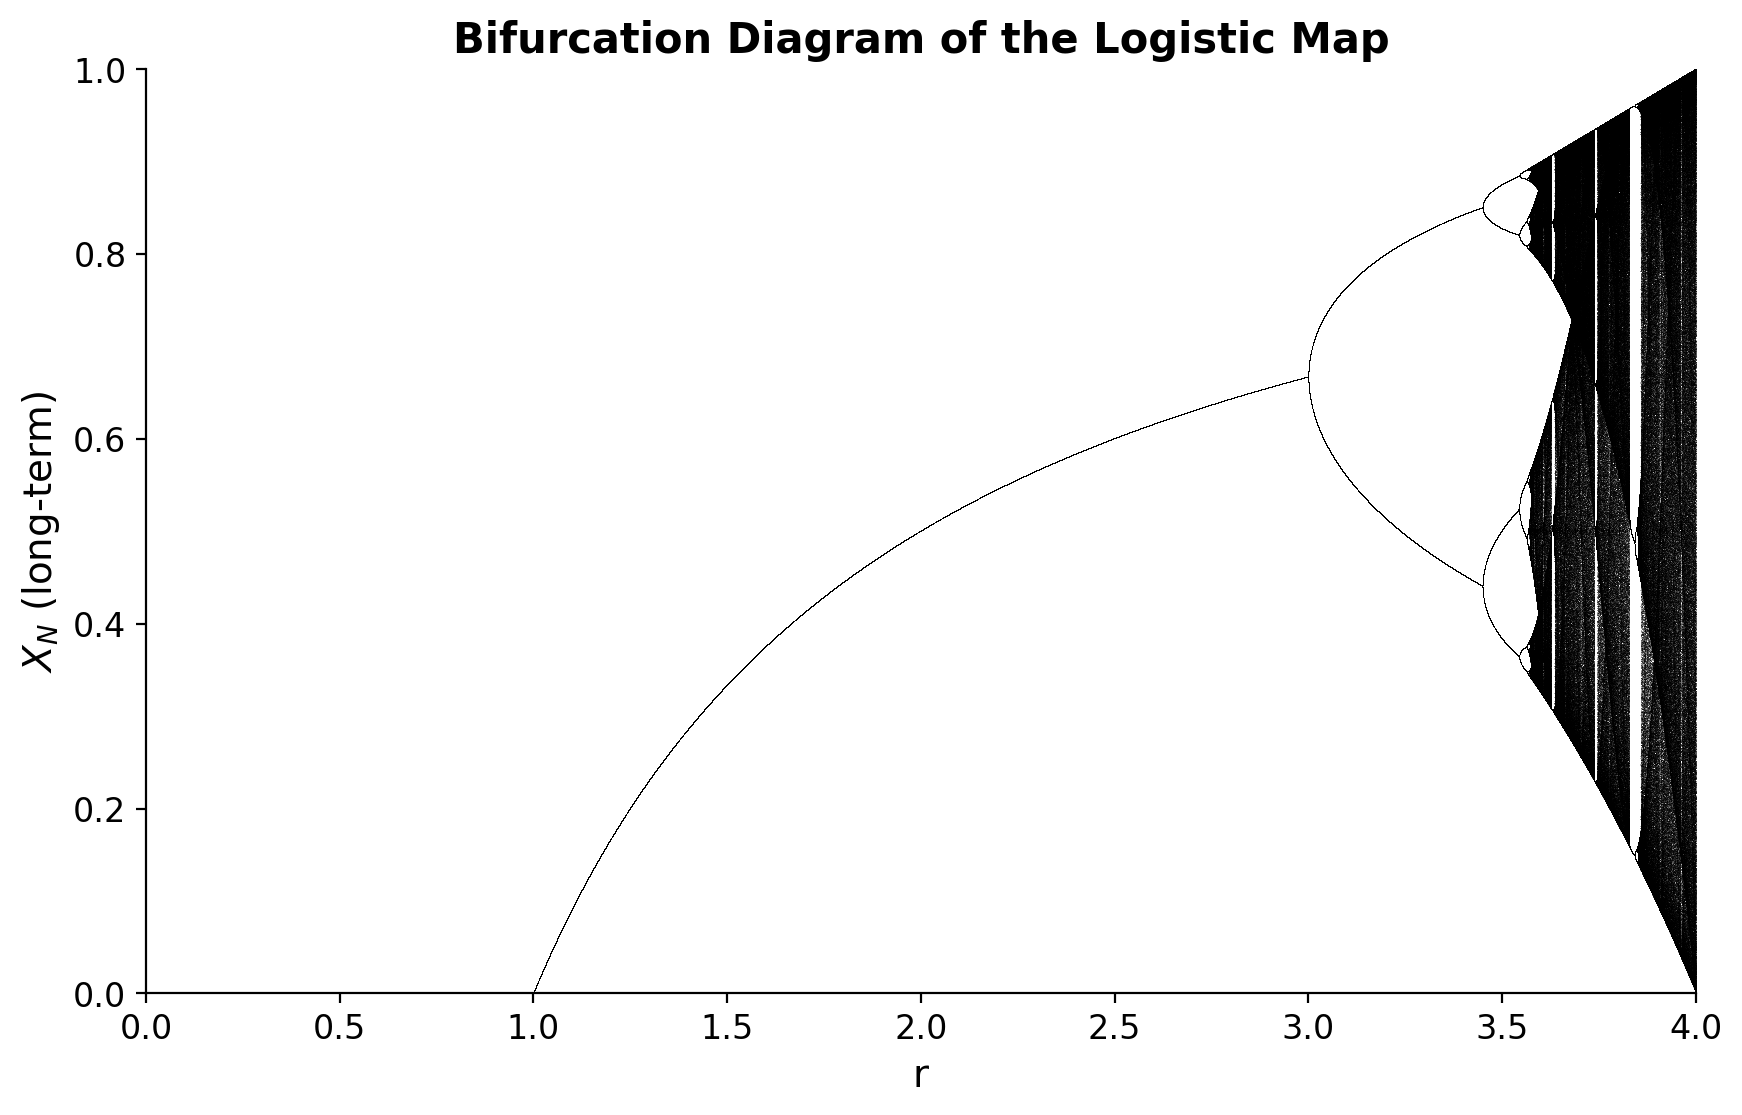
\includegraphics[width=0.82\textwidth]{images/bifurcation_diagram.pdf}
  \end{center}
\end{frame}

\begin{frame}{Reading the Bifurcation Diagram}
  \begin{itemize}
    \item The diagram reveals:
    \begin{itemize}
      \item Single stable branches (fixed points)
      \item Period-doubling cascades
      \item Dense chaotic bands
      \item Windows of order within chaos
    \end{itemize}
    \pause
    \item The ratio between successive bifurcation intervals approaches the \textbf{Feigenbaum constant} $\delta \approx 4.66920$.
    \item This constant is \textbf{universal} --- it appears in many different systems that undergo period-doubling.
  \end{itemize}
\end{frame}

% ---- TikZ: Period-doubling schematic ----
\begin{frame}{Period-Doubling Cascade}
  \begin{center}
  \begin{tikzpicture}[
      level distance=1.4cm,
      sibling distance=2.5cm,
      every node/.style={draw, circle, minimum size=6mm, inner sep=1pt, font=\small},
      edge from parent/.style={draw, thick, -stealth},
      level 1/.style={sibling distance=5cm},
      level 2/.style={sibling distance=2.5cm},
      level 3/.style={sibling distance=1.2cm},
    ]
    \node[fill=primary!20] {1}
      child { node[fill=primary!30] {2}
        child { node[fill=primary!40] {4}
          child { node[fill=secondary!40] {8} }
          child { node[fill=secondary!40] {8} }
        }
        child { node[fill=primary!40] {4}
          child { node[fill=secondary!40] {8} }
          child { node[fill=secondary!40] {8} }
        }
      }
      child { node[fill=primary!30] {2}
        child { node[fill=primary!40] {4}
          child { node[fill=secondary!40] {8} }
          child { node[fill=secondary!40] {8} }
        }
        child { node[fill=primary!40] {4}
          child { node[fill=secondary!40] {8} }
          child { node[fill=secondary!40] {8} }
        }
      };
    \node[draw=none, below=3mm, font=\normalsize] at (0,-5.2) {Period 1 $\to$ 2 $\to$ 4 $\to$ 8 $\to$ \ldots $\to$ \textbf{Chaos}};
  \end{tikzpicture}
  \end{center}
  \vspace{-2mm}
  \begin{itemize}
    \item Each node splits into two at a bifurcation point.
    \item Successive intervals shrink by the Feigenbaum ratio $\delta \approx 4.669$.
  \end{itemize}
\end{frame}

\begin{frame}{Properties of Chaos}
  \begin{itemize}
    \item \textbf{Determinism}: Each state is completely determined by the previous state. There is no randomness --- the system produces its own irregularity.
    \pause
    \item \textbf{Sensitivity to initial conditions}: Tiny differences in $X_0$ grow exponentially over time. This is the famous ``butterfly effect.''
    \pause
    \item \textbf{Aperiodicity}: The sequence never exactly repeats. If it did, determinism would force it to repeat forever --- making it periodic.
    \pause
    \item \textbf{Unpredictability}: Despite being deterministic, long-term prediction is practically impossible because of sensitivity to initial conditions.
  \end{itemize}

  \vfill
  \begin{quote}
    \textit{``Does the flap of a butterfly's wings in Brazil set off a tornado in Texas?''}\\
    --- Edward Lorenz, 1972
  \end{quote}
\end{frame}

\begin{frame}{Sensitivity to Initial Conditions}
  Two trajectories starting at $X_0 = 0.5000000$ and $X_0 = 0.5000001$:
  \begin{center}
    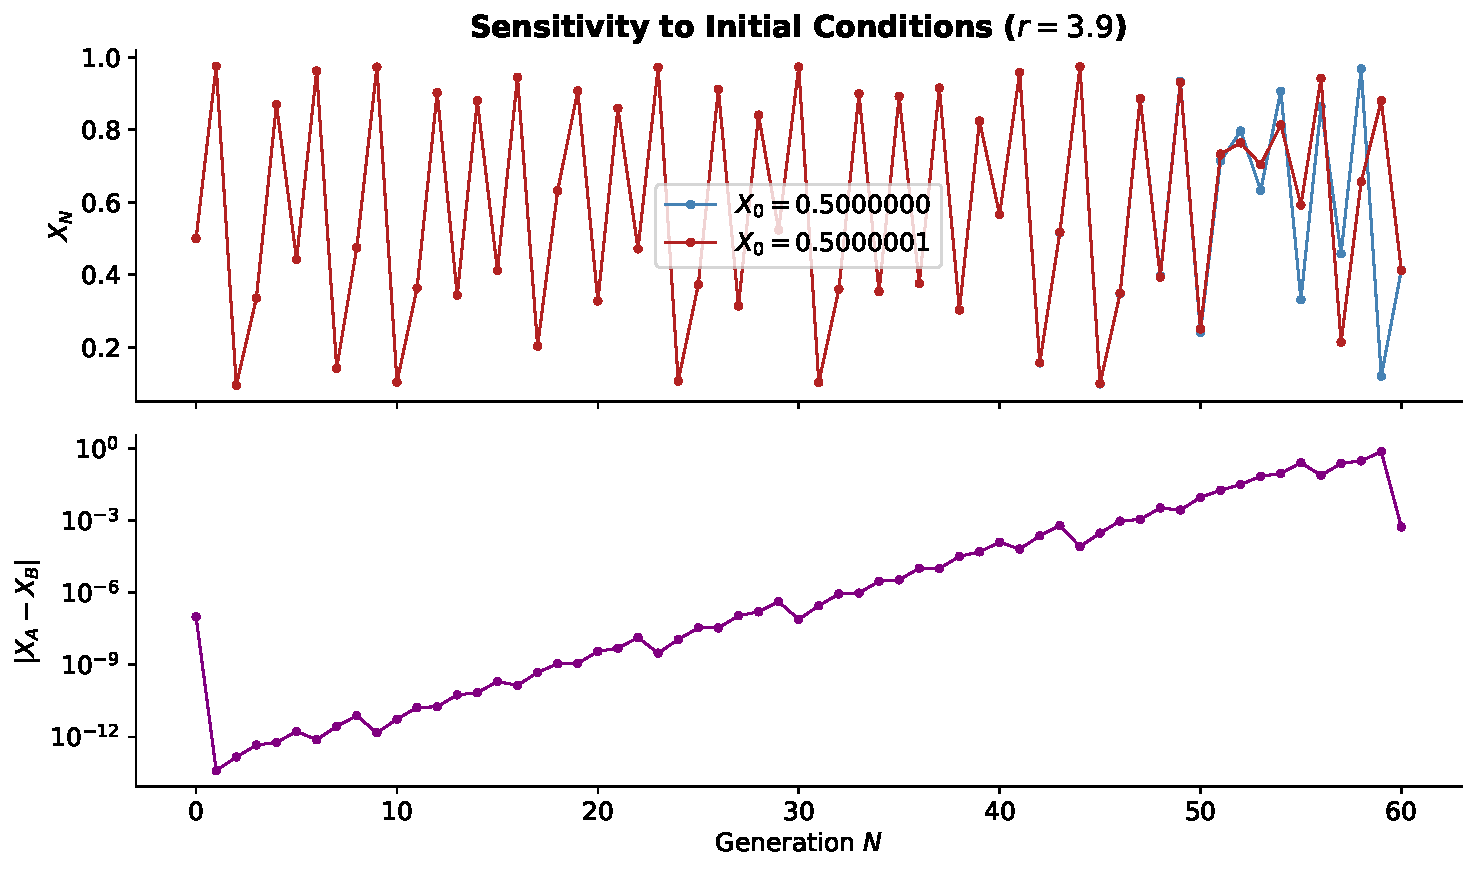
\includegraphics[width=0.85\textwidth]{images/logistic_sensitivity.pdf}
  \end{center}
  \small
  After $\sim$20 generations the tiny initial difference has grown to order~1.
\end{frame}
